\documentclass[12ptletterpaper]{paper}
%this is where the images come from
\usepackage{graphicx}
\graphicspath{ {images/} }
%tab command
\newcommand\tab[1][1cm]{\hspace*{#1}}
\setlength{\oddsidemargin}{-0.25in} % Left margin of 1 in + 0 in = 1 in
\setlength{\textwidth}{7in}   % Right margin of 8.5 in - 1 in - 6.5 in = 1 in
\setlength{\topmargin}{-.75in}  % Top margin of 2 in -0.75 in = 1 in
\setlength{\textheight}{9.2in}  % Lower margin of 11 in - 9 in - 1 in = 1 in
\linespread{1.5}
\usepackage{indentfirst}
\usepackage[authordate]{biblatex-chicago}
\usepackage[bottom]{footmisc}
\usepackage{hyperref}
%this is for quotations
\usepackage{epigraph}
\hypersetup{
	colorlinks,
	citecolor=black,
	filecolor=black,
	linkcolor=black,
	urlcolor=black
}
% --- create title format ---
\title{
	\begin{center}
		\normalfont \normalsize
		\rule{\linewidth}{.5pt} \\[0.4cm] 
		\huge {WinHex} \\ 
		\small{Chris P David}\\
		{\today}\\
		{CSC 317}\\
		{Professor MacDonald}
		\rule{\linewidth}{.5pt} \\
	\end{center}
}
% --- end title format ---


\begin{document}
	\begin{titlepage}
		\clearpage
		\maketitle
		\thispagestyle{empty}
	\end{titlepage}
	\pagebreak	
	\tableofcontents
	\begin{flushleft}
		\pagebreak
		\section{Introduction}
		\tab Essentially in the start sector (or the first sector) we see the MBR. What this does is tell or gives the file system to access the volume. Within this boot sector are is a table with fields that hold many values. Below is an explanation of the offsets followed by what is represented by that offset value.\\
		\tab Almost all of the data shown in this report was taken from some sites, which I will be referencing. For the table in the next section. I will be giving the offset hex value along with the value title, length in bytes if applicable, and lastly the hex value. I also converted the hex value to decimal for items I thought were more suited for a number based answer.
		
		\section{Start Sector }
		
		
		The values are as follows:\\
		At \textbf{offset 0} is the JMP instruction with is basically in every boot record.\\
		At \textbf{offset 3} is the OEM identifier, this is an eight-byte asci string that shows the system that formatted the disk.\\
		At \textbf{offset B} is Bytes per sector, this is the size of a hardware sector.\\
		At \textbf{offset D} is Sectors per cluster, because FAT is limited in the number of clusters it can track, volumes are helped by the ability to increase the numbers of sectors per cluster.\\
		At \textbf{offset E} is Reserved sectors, basically these are sectors that precede the start of the first FAT.\\
		At \textbf{offset 10} is Number of FATs, this is the number of copies of the FAT table on the disk.\\
		At \textbf{offset 11} is Root Entries, this is the total number of file name entries that can be stored in the root directory of the volume.\\
		At \textbf{offset 13} is the Number of Sector, this is used to store the number of sectors on the disk if the volume size is small enough.\\
		At \textbf{offset 15} is Media Descriptor, this byte provides information about the media being used.\\
		At \textbf{offset 16} is Sectors per FAT, this shows the numbers of sectors being occupied by each of the FATs on volume. \\
		At \textbf{offset 18} is Sectors per Head, these values are a part of the disk geometry in use when the disk was formatted.\\
		At \textbf{offset 1A} is Heads per Cylinder, like Sectors per head these values are a part of disk geometry, though these reflect the number of cylinders per head\\
		At \textbf{offset 1C} is Hidden Sectors, is the number of sectors on the physical disk preceding the start of the volume, before the boot sector itself\\
		At \textbf{offset 20} is Big number of Sectors, basically this is an indicator if the small sectors field is either zero or nonzero.\\
		At \textbf{offset 24} is Big Sectors Per FAT, this is related to the BIOS physical disk number.\\
		At \textbf{offset 28} is ExtFlags, a check for is if the FAT is in synch or not. Also for if FAT mirroring is disabled.\\
		A Note the following fields are only defined for FAT32.\\
		At \textbf{offset 2A} is FSVersion, version of file system.\\
		At \textbf{offset 2C} is RootDirectoryStart, contains the number of the first cluster for the root directory.\\
		At \textbf{offset 30} is FSInfoSector, this is the number for the file system information sector.\\
		At \textbf{offset 32} is BackupBootSector, this is the sector number for the backup copy of the boot sector.\\
		At \textbf{offset 34} is Reserved, reserved.\\
		All information taken from \footnote[1]{\hyperlink{Detailed Explanation of the FAT Boot Sector}{Detailed Explanation of the FAT Boot Sector}}.
		\subsection{WinHex Table}
		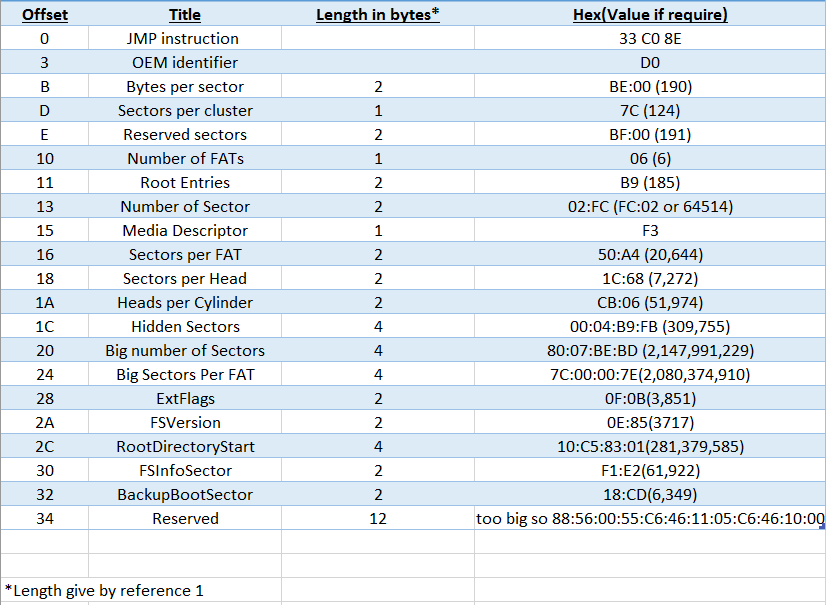
\includegraphics{graph.png}
		
		\section{Slack Space File}
		\textbf{File Name}- UNDERTALE.exe\\
		\textbf{File Extension}- EXE\\
		\textbf{Size}- 3.6MB\\
		\textbf{Creation Date}-10/14/2016 16:03\\
		\textbf{Last Modification Date}-06/23/2016 20:36\\
		\textbf{Last Access Date}-10/26/2016\\
		\textbf{Attributes}-A\\
		\textbf{First Sector Number}-53,991,744\\
		\textbf{(First) Cluster Number}-1,686,220\\
		\textbf{Physical Sector Number}-53,991,744\\
		\textbf{Logical Sector Number}-53,991,776\\
		
		\tab The size of the file is 3.6 MB which is roughly 3774873 bytes.\\
		\tab Current Cluster number is 1,689,769 -> 1,689,770.\\
		\tab I then saved the block of slack space in my directory for this class.\\
		
		\pagebreak
		\section{Bibliography}
		
		\noindent\hypertarget{Detailed Explanation of the FAT Boot Sector}{Detailed Explanation of the FAT Boot Sector\\Detailed Explanation of the FAT Boot Sector. Retrieved October 25, 2016,from http://www.dewassoc.com/kbase/harddrives/bootsector} \vspace{12pt}		
		
		
	\end{flushleft}
\end{document}